\subsubsection{CPU使用率の表示}

\begin{enumerate}
\item ログを読み込む
\item OS全体のロード・ロードアベレージを表示する。(\figref{all})
\item ロード・ロードアベレージの横の\fbox{+}がクリックされると、コア別のロード・ロードアベレージを表示する。(\figref{core})
\item コア別のロード・ロードアベレージの横の\fbox{+}がクリックされると、優先度別のロード・ロードアベレージを表示する。
\end{enumerate}

\begin{figure}
\centering
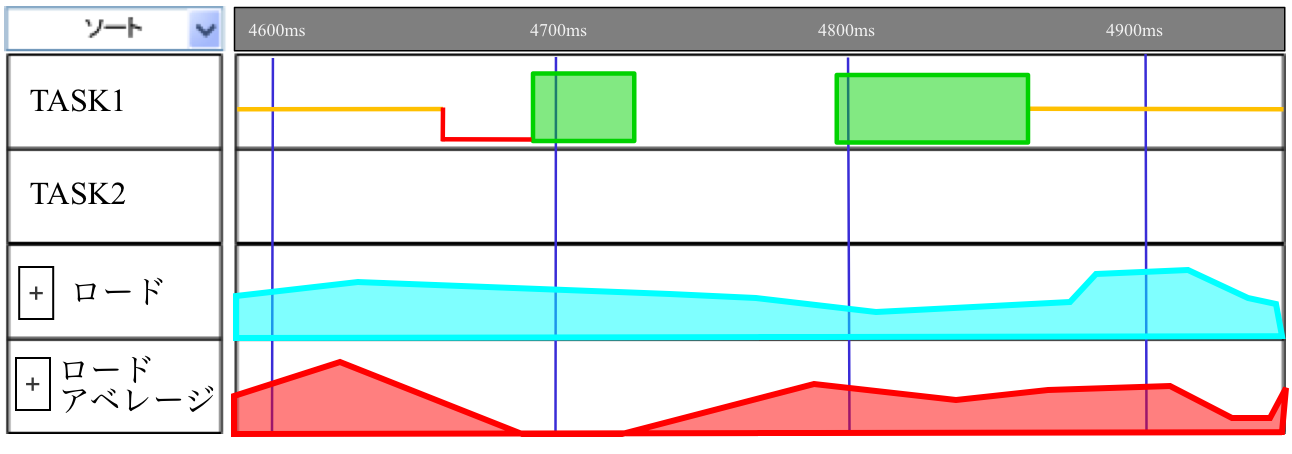
\includegraphics[width=10cm]{all.png}
\caption{OS全体のロード・ロードアベレージ表示}\label{all}
\end{figure}

\begin{figure}
\centering
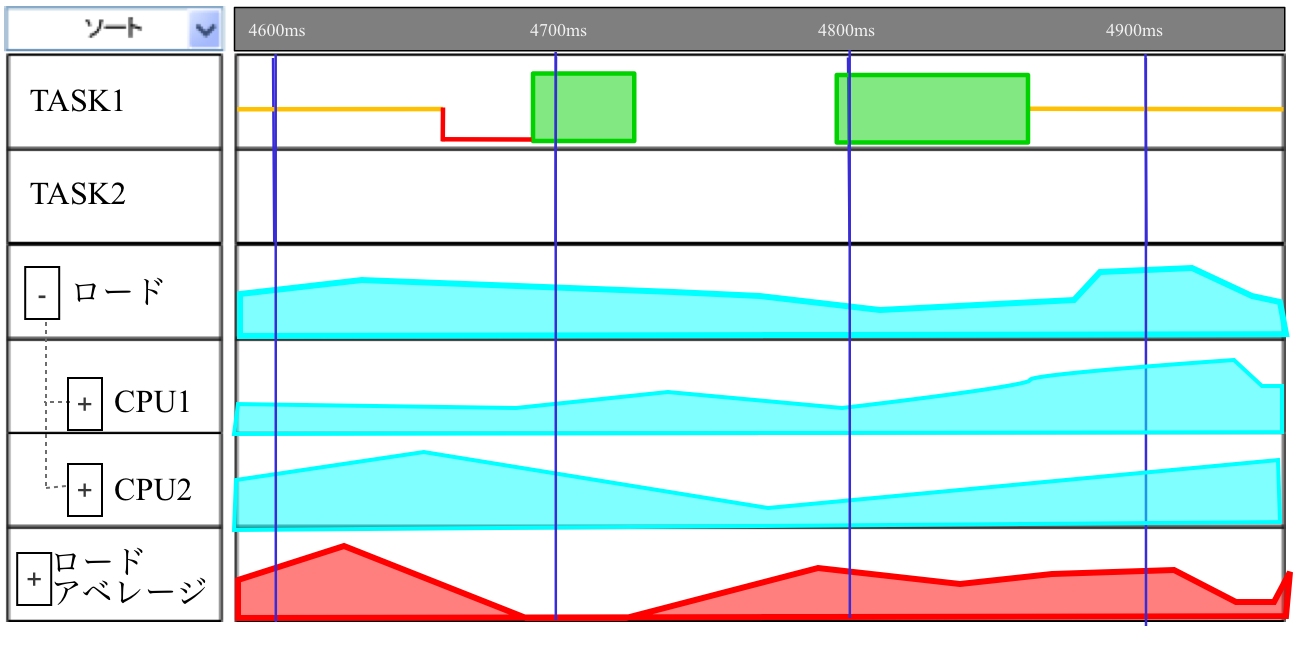
\includegraphics[width=10cm]{core.png}
\caption{コア別のロード・ロードアベレージ表示}\label{core}
\end{figure}

\begin{figure}
\centering
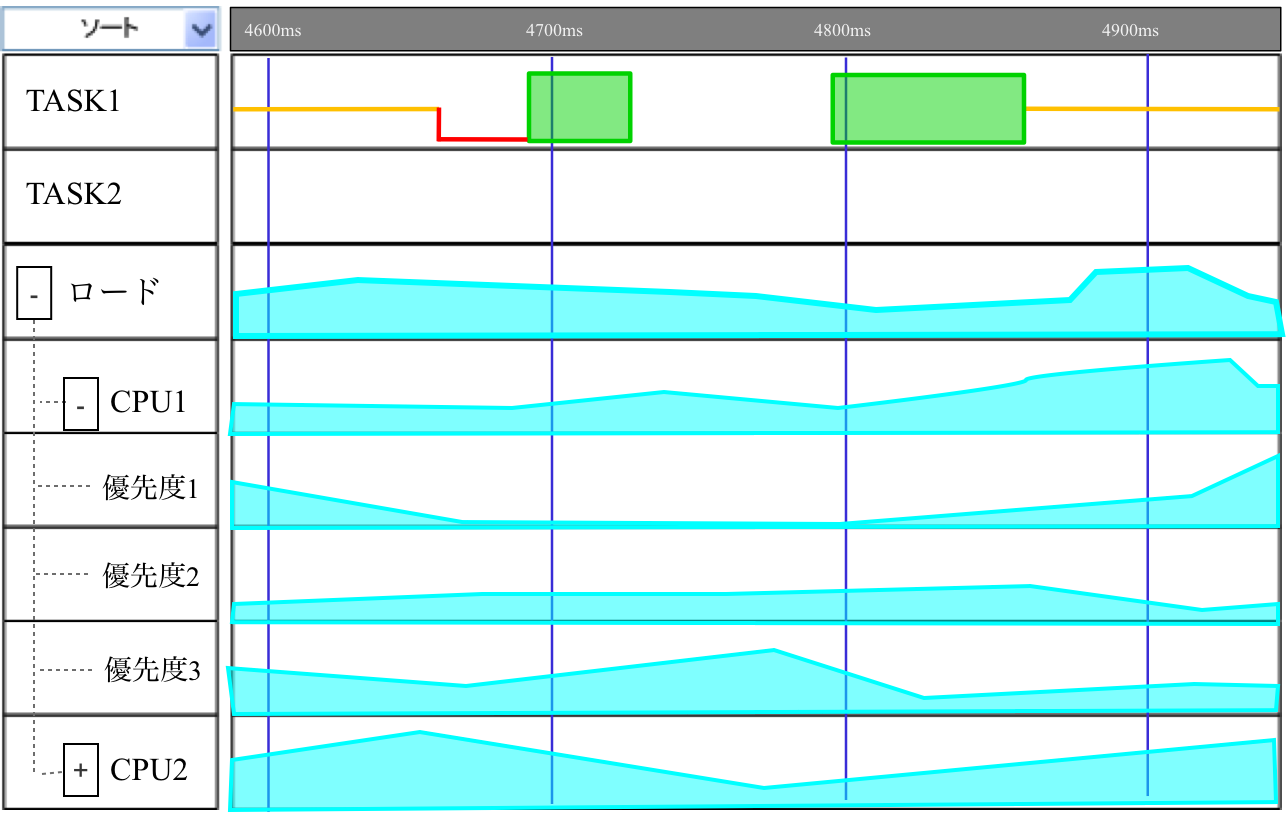
\includegraphics[width=10cm]{pri.png}
\caption{優先度別CPU使用率表示}\label{pri}
\end{figure}
